\newsection
\subsection{Inequity and fairness}
\label{sec:fairness}
\sectionauthors{Rishi Bommasani, Fereshte Khani, Esin Durmus, Faisal Ladhak, Dan Jurafsky}

\begin{figure}[!ht]
    \centering
    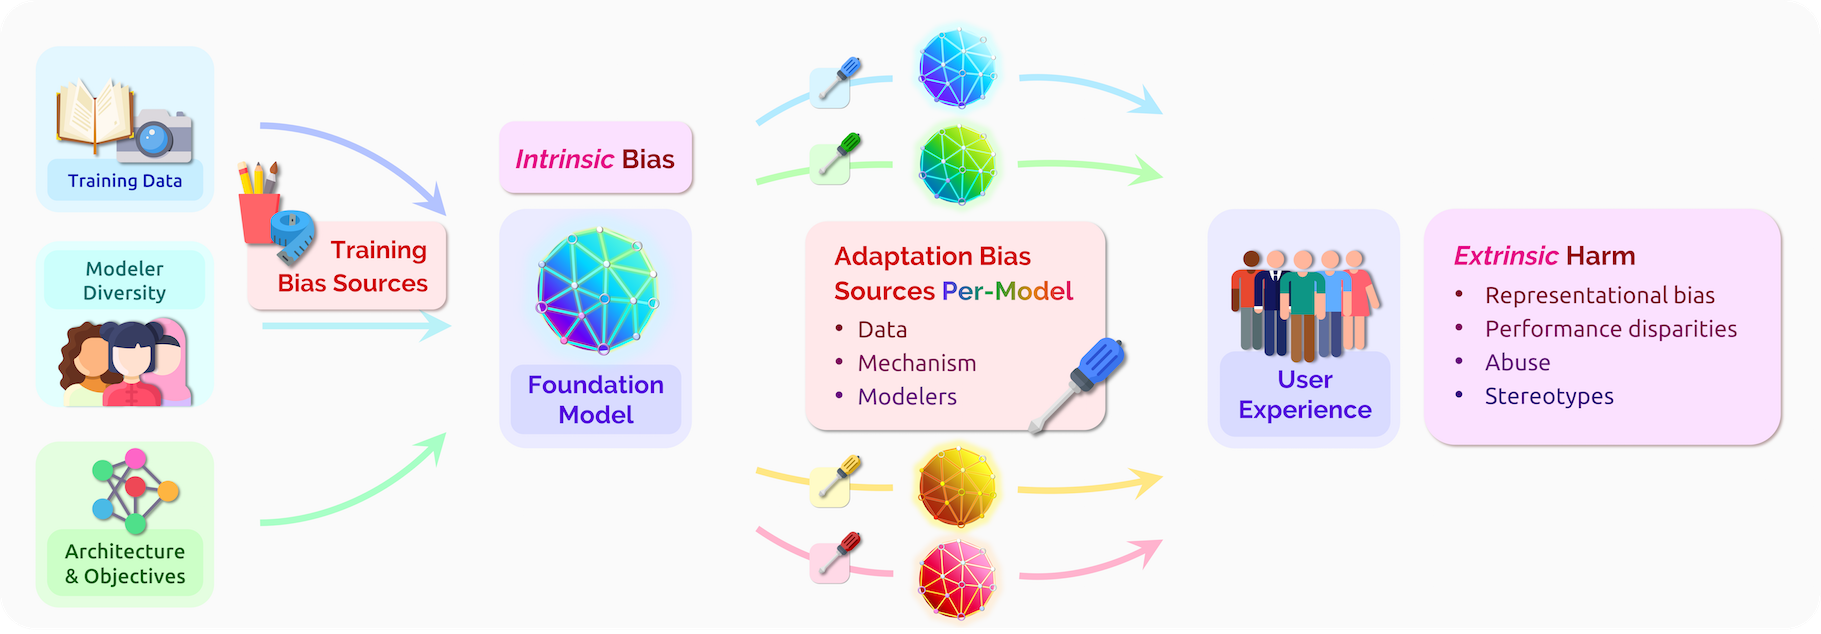
\includegraphics[width=\linewidth]{society/figures/Inequity.png}
    \caption{The \textit{intrinsic bias} present within foundation models is the byproduct of various training bias sources (\textbf{left}) which, alongside biases introduced during adaptation, determines the \textit{extrinsic harms} (\textbf{right}) experienced by users in the context of specific downstream applications. We emphasize that the same foundation model is the shared foundation for many different applications; its biases pervade to these many applications as a result. Further, since the harms experienced by users are the result of specific adapted models, attributing these harms to the various processes and sources depicted in this diagram is both crucial and challenging.}
    \label{fig:fairness}
\end{figure}

\subsubsection{Introduction}
\label{sec:fairness-introduction}
Foundation models have the potential to yield inequitable outcomes: the treatment of people that is unjust, especially due to unequal distribution along lines that compound historical discrimination \citep{Hellman2021Big}. Like any AI system, foundation models can compound existing inequities by producing unfair outcomes, entrenching systems of power, and disproportionately distributing negative consequences of technology to those already marginalized \citep{sweeney2013,kay2015,buolamwini2018gender,benjamin2019,ajunwa2019paradox,datafeminism,crawford2021}. 
Here we ask what fairness-related harms relate to foundation models, what sources are responsible for these harms, and how  we can intervene to address them. 
The issues we discuss here are related to  broader questions of algorithmic fairness and AI ethics \citep{CorbettDavies2018, Chouldechova2020, Hellman2020, Johnson2020, fazelpour2021bias}, race and technology \cite{benjamin2019, Hanna2020, Gebru2021, field2021}, and the coexistence of society and technology \citep{Abebe2020}.

\subsubsection{Harms}
\label{sec:fairness-harms}
Foundation models are intermediary assets with no specified purpose before they are adapted; understanding their harms requires reasoning about both their properties and the role they play in building task-specific models. 
We delineate \textit{intrinsic} biases,\footnote{We use the word \textit{bias} to denote the properties of a foundation model that contribute to inequity; we follow \citet{blodgett_language_2020} in attempting, when possible, to delineate who is harmed and how they are harmed.} \ie~properties of the  foundation model that indirectly but pervasively affect downstream applications, and \textit{extrinsic harms}, \ie~harms that arise in the context of specific downstream applications \citep{galliers1993}.

\paragraph{Intrinsic biases.}
Properties of the foundation model can lead to harm in downstream systems.
As a result, these intrinsic biases can be measured directly within the foundation model, though the harm itself is only realized when the foundation model is adapted, and thereafter applied, \ie~these are \textit{latent} biases or harms \citep{DeCamp2020}.
We focus on the most widely studied form of intrinsic bias, \textbf{representational bias}, specifically considering misrepresentation, underrepresentation and overrepresentation. 
People can be \textbf{misrepresented} by pernicious stereotypes \citep{bolukbasi2016, caliskan2017, abid2021,stereoset,gehman-etal-2020-realtoxicityprompts} or negative attitudes \citep{hutchinson2020}, which can propagate through downstream models to reinforce this misrepresentation in society \cite{noble,benjamin2019}. 
People can be \textbf{underrepresented} or entirely erased, \eg~when LGBTQ+ identity terms  \citep{Strengers2020, Oliva2021, Tomasev2021} or data describing African Americans \cite{buolamwini2018gender,koenecke2020racial,blodgett17} is excluded in training data, downstream models will struggle with similar data at test-time.
People can be \textbf{overrepresented}, \eg~BERT appears to encode an Anglocentric perspective \citep{zhou2021} by \textit{default}, which can amplify majority voices and contribute to \textit{homogenization} of perspectives \citep{creel2021} or monoculture \citep{kleinberg2021} (\refsec{ethics}). 
These representational biases pertain to all AI systems, but their significance is greatly heightened in the foundation model paradigm.
Since the same foundation model serves as the basis for myriad applications, biases in the representation of people pervade to many applications and settings.
Further, since the foundation model does much of the heavy-lifting (compared to adaptation, which is generally intended to be lightweight), we anticipate that many of the experienced harms will be significantly determined by the internal properties of the foundation model.

\paragraph{Extrinsic harms.}
Users can experience specific harms from the downstream applications that are created by adapting a foundation model.  
These harms can be \textbf{representational}  \citep{barocas17,crawford17,blodgett_language_2020}, such as the sexualized depictions of black women produced by information retrieval systems \citep{noble}, the misgendering of persons by machine translation systems that default to male pronouns \cite{schiebinger13,schiebinger14}, or the generation of pernicious stereotypes \citep{nozza21,sheng-etal-2019-woman, abid2021}. 
They can consist of \textbf{abuse}, such as when dialogue agents based on foundation models attack users with toxic content \cite{dinan21,gehman-etal-2020-realtoxicityprompts} or microaggressions \citep{breitfeller-etal-2019-finding,jurgens-etal-2019-just}.
All of these user-facing behaviors can lead to psychological harms or the reinforcement of pernicious stereotypes \cite{spencer2016stereotype,williams2020psychology}.

In addition to harms experienced by individuals, groups or sub-populations may also be subject to harms such as group-level \textbf{performance disparities}.
For example, systems may perform poorly on text or speech in African American English \citep{blodgett17,koenecke2020racial}, incorrectly detect medical conditions from clinical notes for racial, gender, and insurance-status minority groups \citep{zhang2020hurtful}, or fail to detect the faces of people with darker skin tones \citep{wilson19,buolamwini2018gender}. 
As foundation models are more pervasively applied, including in high-stakes domains, these disparities can spiral into further, and more severe, harms. 
\citet{koenecke2020racial} discuss how if African American English speakers cannot reliably use speech recognition technologies (\eg~due to inequities in underlying foundation models), this may mean they cannot benefit from certain derivative products (\eg~voice assistants, assistive technologies) and will be disadvantaged if these technologies are used to conduct interviews for employment or transcribe courtroom proceedings.
More generally, characterizing these group-level harms (and working towards justice for those harmed) also requires the AI community to improve its understanding of group-based prejudice \citep{allport1954} and social groups: we point to relevant work in the social sciences and other communities on moving beyond binary treatments of gender \citep{lindsey2015, westbrook2015, richards2017, darwin2017, Keyes2018, hyde2019, cao2020, dinan2020}, more nuanced treatments of race \citep[\eg][]{penner2008, freeman2011,  saperstein2012, saperstein2013, penner2015, field2021}, better addressing intersectional identities \citep[\eg][]{crenshaw1989, nash2008, gines2011, penner2013, ghavami2013, bright2016, buolamwini2018gender, may2019, oconnor2019, guo2020}, and more modern treatments of disability \citep[\eg][]{batterbury2012, spiel2019, hutchinson2020}. 

\paragraph{Additional considerations.}
To more completely understand the harms of foundation models, further \textit{documentation} is required of both the intrinsic biases and extrinsic harms; future work should articulate the relationship between intrinsic biases and extrinsic harms \citep{blodgett_language_2020, blodgett2021, goldfarb-tarrant2021}.
This documentation requires centering stakeholders beyond academics and industry practitioners: the inequitable impact of foundation models will be experienced largely by minority populations, which are underrepresented in both academia and industry. 
For foundation models specifically, their creation and study likely will be conducted by those with the access and resources required, further emphasizing the importance of venues that center marginalized voices \citep[][\refsec{ethics}]{datafeminism}.
In particular, user studies of specific adapted models, when aggregated across applications, can provide compelling and individualized documentation of the harms that derive from the intrinsic biases of foundation models, all while centering individual users.
In this way, we imagine the methodologies in human-computer interaction (HCI), with some adjustment to accommodate the abstraction involved in foundation models, will help center the voices of marginalized communities (further discussion in \refsec{interaction}). 

\subsubsection{Sources}
\label{sec:fairness-sources}
In order to fully characterize and properly intervene on the harms of foundation models, we must be able to trace their source to the properties of the foundation model and the adaptation process, and further decompose to the roles of individual sources of biases \citep{friedman1996}. 
Source tracing is vital for attributing ethical and legal responsibility for experienced harm, though attribution will require novel technical research that foregrounds matters such as causality \citep{pearl2000causality} and influence \citep{koh2017understanding}.

\paragraph{Data.}
Data of several types shapes the behavior of applications, and the associated extrinsic harms, based on foundation models: the training data used to train the foundation model, the adaptation data used to adapt the foundation model, and test-time user data/interaction.
For all of these data sources, the properties of the data (\eg~toxicity and hate speech \citep{henderson17ethical},  abusive language \citep{waseem-etal-2017-understanding}, microaggressions \citep{breitfeller-etal-2019-finding}, stereotypes \citep{voigt-etal-2018-rtgender}) will manifest in the biases of the foundation model (and its adapted derivatives).\footnote{In adaptation, which involves labelled task-specific data, biases in the choices of the label space \cite{crawford2021} and biases in the annotators who label that data \citep{geva-etal-2019-modeling,sap-etal-2019-risk} can also contribute to extrinsic harms experienced by users.}
Since the training data is the key data source that determines the foundation model and the associated intrinsic biases, we focus on the training data here.
At present, the relationship between the training data, along with associated data practices (\eg~data curation, data selection, and data weighting \citep{paullada2020, bender2021, rogers2021}) and the intrinsic biases acquired by the foundation model remains unclear; future work is critically needed to clarify this relationship.
Since foundation models generally require training data of immense scale, which poses clear challenges not only to its documentation \citep{bender2021} but also comprehensive scientific exploration to articulate the relationship of data biases and model biases, we anticipate new protocols are required to address this scale.
Establishing scaling laws for bias, akin to those for accuracy metrics \citep{kaplan2020, henighan2020}, may enable systematic study at smaller scales to inform data practices at larger scales.

\paragraph{Modeling.} 
Modeling decisions (\eg~training objective (\refsec{training}), model architecture (\refsec{modeling}), adaptation method (\refsec{adaptation}))  influence the biases in foundation models and their derivatives, thereby affecting the experienced extrinsic harms.  
Existing work demonstrates the foundation models amplify training data biases, extending trends seen for machine learning and deep learning models \citep{zhao-etal-2017-men,wang2019balanced,jia-etal-2020-mitigating,hashimoto2018fairness}, though much still remains unclear about what and how model properties are responsible for this bias amplification.
Further, given that applying foundation models directly may be infeasible (due to their scale), efforts to compress these models or make them more efficient also appear to amplify bias \citep{hooker2020, renduchintala2021}.
Amplification may also be exacerbated by feedback loops, in which foundation models modify societal behavior and induce sociological changes, which modifies subsequent training data; feedback effects of this form tend to exacerbate inequity in other  ML applications \cite{lum2016predict,ensign2018runaway,hashimoto2018fairness}.
Beyond the explicit decisions made in training and applying foundation models, community values \citep{birhane2020} and norms (\refsec{ethics}) both indirectly and implicitly \citep{liu2021} shape decision-making in building models.
As a result, measuring biases in conjunction with work introducing foundation models \citep[\eg][]{brown2020gpt3} and in standard benchmarks \citep[][\refsec{evaluation}]{friedman1996}, as well as conducting user studies with diverse user groups to document experienced harm, are steps towards ensuring best practices actively emphasize the consideration of bias and inequity.
\paragraph{Modelers.}
As with all algorithmic systems, poor representation and diversity of stakeholders and marginalized communities in decision-making bodies that develop or apply foundation models is inherently problematic, and may contribute to greater experienced harm for these communities.\footnote{We note that diversity, both with respect to disciplinary backgrounds and demographic identities, is of fundamental importance in these high-impact decision-making settings for reasons well beyond the potential improved recognition of fairness-related harms.} 
While difficult to document, existing efforts to develop foundation models suggest this as a possibility: 
\citet{caswell2021} demonstrate the flawed data handling of less-represented languages in the multilingual datasets used to train multilingual models and \citet{hutchinson2020} show that models often contain undesirable biases towards disabled persons. 
In both instances, these biases and harms may have been noticed earlier by better representation of these parties in developer teams. 
Further, since end-users are likely more diverse than developers and may notice these concerns earlier, allowing for user feedback to contribute to foundation model design (\refsec{interaction}) is an important direction forward.

\subsubsection{Interventions and recourse}
\label{sec:fairness-recourse}

Addressing, mitigating, and rectifying the inequities associated with technology requires  integrating social and technical methodologies \citep{Abebe2020}.
 For foundation models specifically, we consider both proactive methods, which change how models are developed and deployed to prophylactically reduce harm, as well as reactive methods, which respond to harm and make changes for the future.
 At its core, the abstraction of foundation models complicates both aspects: knowing if interventions at the level of the foundation level are successful in reducing harm requires downstream observations at the level of specific deployed applications and recourse in the event of harm requires upstream propagation of both feedback and accountability to foundation model providers.
 
\paragraph{Intervention.}
General principles that govern intervention on technological systems apply to the foundation model setting: identifying which sources are most responsible for bias or harm provides the evidence required for targeted action.
For example, the urgency of calls for improved diversity in the teams that design, produce, and control technology (\eg~foundation models) and their applications \citep{Longino1990, Harding2015, Nielsen2017, oconnor2019, Hofstra2020, Katell2020} is further intensified if the lack of diversity is shown to relate to harm \citep{caswell2021}. 
In addition, transparent documentation \citep[\eg][]{gebru2018datasheets, bender2018data, Mitchell_2019} and auditing \citep[\eg][]{raji2019} are similarly critical in providing the impetus for intervention and change \citep{Burrell2016, Lipton2018, Creel2020, Raji2020, Wilson2021}.
The scale of foundation models, as well as the specifics of their accessibility, introduce new challenges for existing protocols for documentation and auditing that we discuss further in \refsec{ethics}.

To date, many of the interventions considered for reducing the inequitable impact of technology, including in the foundation model regime, are methods for technical mitigation that center the data (to obviate reflecting inequities or biases) and modelling decisions (to avoid amplifying data biases) involved.
Of specific importance in the foundation model regime is recognizing that these mitigation approaches may target different steps in the pipeline such as the training data \citep[\eg][]{lu2020}, modelling objectives \citep[\eg][]{zhao2018}), and adaptation methods and test-time use \citep[\eg][]{park2018,zhao2019}.
As a result, different approaches may not only be more or less effective, but require action from different entities (\eg~foundation model providers vs. application developers) and more or less intensively affect the expensive training process for these models (\eg~changing the process of creating a foundation model vs. altering it \textit{post hoc}).
Technical intervention of this form may also target different goals: some interventions, such as changing the training data, aims to reduce \textit{intrinsic bias}.
One the other hand, most work on mitigation in algorithmic/ML fairness instead considers reducing outcome disparities in terms of model behavior, \ie~the outputs of downstream systems that more directly relate to \textit{extrinsic harm}. 
Technical mitigation of all forms at present is severely limited: methods that measure or combat intrinsic bias are brittle or ineffectual \citep{gonen19, ethayarajh2019, bommasani2020, zhou-etal-2021-challenges, Antoniak2021}, methods that measure or combat extrinsic outcome disparities may not align with stakeholder goals \citep{saha2020}, and there is some evidence to suggest certain types of technical intervention may be simultaneously unsatisfiable \citep{CorbettDavies2018, kleinberg2017}, impossible \citep{lechner2021}, or may even exacerbate inequity \citep{xu-etal-2021-detoxifying}.
In spite of this state of affairs, we continue to believe technical methods will still play an instrumental role in addressing the harms that arise in the foundation model regime; in general, we advocate for transparency, especially given that technical mitigation methods may not be able to achieve the intended goals.
More broadly, claims of bias and bias mitigation must be made carefully to clearly communicate the status quo to various stakeholders with differing expertise (\eg~application developers building on top of foundation models and policymakers regulating the technology; \citep{nissim2020}). 

\paragraph{Recourse.}
Unfortunately, proactive intervention is unlikely to full resolve all potential harm or inequity that may arise due to foundation models.
When harm arises, there is currently no widely-adopted (or legally required) framework for resolving the appropriate recourse for the harmed parties.
While certain protocols may exist for specific applications, the abstraction of foundation models again introduces a disconnect: harms likely are partially attributable to both the foundation model providers and the downstream application developers, but allocating this responsibility to either party remains challenging.
More simply, mechanisms are not in place to even communicate these harms to foundation model providers (even if feedback or complaints are raised to application developers).
As a result, new norms and standards are needed on  how  feedback from  application developers and end-users should reach upstream to the foundation model providers, how to determine the entities (\eg~foundation model providers, application developers) responsible for these harms, and the relationship to legal responsibility (\refsec{legality}).
To make progress on this matter, we encourage future work to consult the practices used in other domains (especially those with similar abstractions and multi-entity structures), and we anticipate any standards introduced will likely need to be reasonably dynamic, so that they can be synchronized with the rapidly changing status quo for these models and their applications.

\subsubsection{Takeaways}
\label{sec:fairness-takeaways}
Machine learning has an established trackrecord of inequitable impact, with much of the burden of its harms borne by marginalized communities.
Foundation models introduce new challenges to this calculus but, ultimately, for their societal impact to be equitable, significant research and change is required to understand the harms they cause and to meaningfully address and rectify these harms:
\begin{enumerate}
    \item 
    The one-to-many nature of foundation models, \ie~the same few foundation models being used across many applications, means the intrinsic properties of foundation models pervade to many downstream applications. Pernicious biases in these models therefore have out-sized effect on the experienced harms.
    \item 
    Biases and harms in the foundation model regime originate from many sources (\eg~training and adaptation data, modelling and adaptation decisions, modeler diversity and community values). 
    Attributing the sources for bias and harm is fundamental for questions of intervention and responsibility; attribution requires new technical research to be done reliably.
    \item 
    The inequities of foundation models are not inevitable, but addressing them requires a multi-pronged approach comprised of both proactive intervention (\eg~data-centric and model-centric changes) and reactive recourse (\eg~mechanisms for feedback and accountability).
\end{enumerate}
